\section{Metodologia}\label{sec:methods}

Este Trabalho foi desenvolvido através de pesquisa bibliográfica que fornece subsídios
para empreender as análises referentes à necessidade de implementação de um modelo de
científicos. Nesta pesquisa, quanto aos objetivos, caracteriza-se como descritiva\cite{GIL}
, identificando os possíveis benefícios, funcionalidades e contribuições do
Sistema de Informações, aborda o processo formal e sistemático de desenvolvimento do método científico, sendo seu objetivo fundamental a obtenção de respostas para questões mediante o emprego de procedimentos científicos.Além disso, Segundo \cite{GIL}, “a pesquisa bibliográfica é elaborada com base em material
já publicado”, incluindo [...] “livros, revistas, jornais, teses, dissertações e anais de eventos
científicos”. A pesquisa bibliográfica permite elaborar as informações científicas já existentes,

sistematizando o conhecimento já produzido\cite{LEHFELD} 
 Tendo em vista que a Neuroevolução é uma forma de aprendizado de inteligência artificial,  e consiste em utilizada com algoritmos evolutivos para  melhorar o desempenho de arquiteturas de rede neural, simplificar o processo de resolução de tarefas complexas em domínios como jogos, robótica e simulação de processos naturais.\cite{neuroevolucao}
À partir dessa informação, tem como foco mostrar os conceitos que foram usados para o recriação de um jogo já existente denominado de Flappy Bird, é um jogo eletrônico criado para dispositivos móveis desenvolvido no ano  de 2013 desenvolvido em Hanói Capital do Vietnã, Pelo DESENVOLVEDOR vietnamita Nguyễn Hà Đông e publicado pela .GEARS studios.\cite{CriadorJogo}

A ideia restringe se em recriar o jogo Flappy Bird utilizando \textbf{NEAT} para fazer com que o Agente aprenda sozinho como jogar e zerar o jogo vencendo todas as fases e passando por todos os obstáculos. a escolha do jogo nasceu por ser um jogo simples e de fácil e de rápida criação podendo assim aplicar as técnicas de criação da interface com o Pygame 
Na fase inicial eu utilizei o Pygame  para construir a parte gráfica cálculos de  Largura e Altura de tela e iniciação de fonte  desenho dos elementos em tela. e iniciação de fonte  desenho dos elementos em tela.
Utilização da programação orientada a objetos para criação dos elementos do jogo 
que é o pássaro, cano e chão.
O objeto pássaro é composto de imagens para fazer a animação do bater das asas
\textbf{Contém quatro funções:}
\begin{itemize}
    \item \textbf{Init}
    \begin{itemize}
    \item A função \textbf{init} que é chamada na instanciação do objeto recebendo como parâmetros 
os valores de X e Y que determinam as coordenadas do objeto pássaro no plano cartesiano, dados que vão ser passados para minha rede para tomada de decição do agente.
\end{itemize}


\item \textbf{jump}
    \begin{itemize}
    \item A função Jump controla os valores de velocidade e tempo controlando a variação, e atribui a altura o valor da variável \textbf{Y (Variável que representa o eixo de subida)}  
\end{itemize}

 

\item \textbf{Move}
    \begin{itemize}
    \item A função Move que determina o movimento que consiste em um função MRUV para determinar o deslocamento.\\
S = so + vot + at²/2
 \textbf{Y}
\end{itemize}

\item \textbf{draw}
    \begin{itemize}
    \item A função draw faz animação do bater de asas desenhar a pássaro na tela, através de uma função screen.blit objeto passada por parâmetro na função draw.
\end{itemize}
\end{itemize}

as outras são iniciadas com valores padrão e imagens carrega com um array de imagens para compor a animação do pássaro








%
\subsection{\textbf{Implementação da IA com Neat-Python}}
Vamos analisar a parte dos hiperparâmetros que fica no arquivo \textbf{config.txt}.
A parte mais importante são os parâmetros de rede,
que representa o nosso perceptron ilustrado na imagem abaixo.
Os num inputs são os sensores do agente, onde vai
perceber o ambiente, \textbf{a posição do agente no eixo Y + distância do agente para o cano de cima + distância do pássaro para o cano de baixo = num inputs = 3}, são as informações que vou colocar na rede, 
que no meu caso são 3.
E meu num outputs = 1 pois ação do meu agente é saltar
O parâmetro num hidden = 0 , ele seria o número de camada oculta no entanto isso você aumenta a complexidade da sua rede resultando uma em um tempo maior de convergência falaremos disso em resultado e teste. 
\begin{lstlisting}
# network parameters
num_hidden              = 0
num_inputs              = 3
num_outputs             = 1
\end{lstlisting}

\begin{figure}[htpb!]
    \centering 
    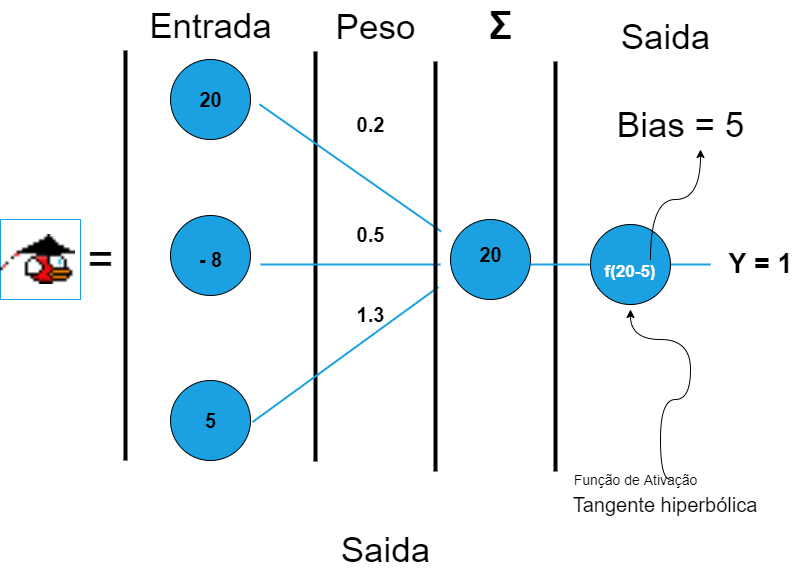
\includegraphics[width=0.7\linewidth]{images/passaroRNA3.png}
    \caption{Perceptron.}
    \label{fig:gym}
\end{figure}
O projeto a qual me inspirei  num imputs = 5 sensores do carro e
num outputs  = 3, pois há 3 ações. virar a esquerda, virar a direita, e aceleração.
O parametro num hidden = 0.
\begin{figure}[htpb!]
    \centering 
    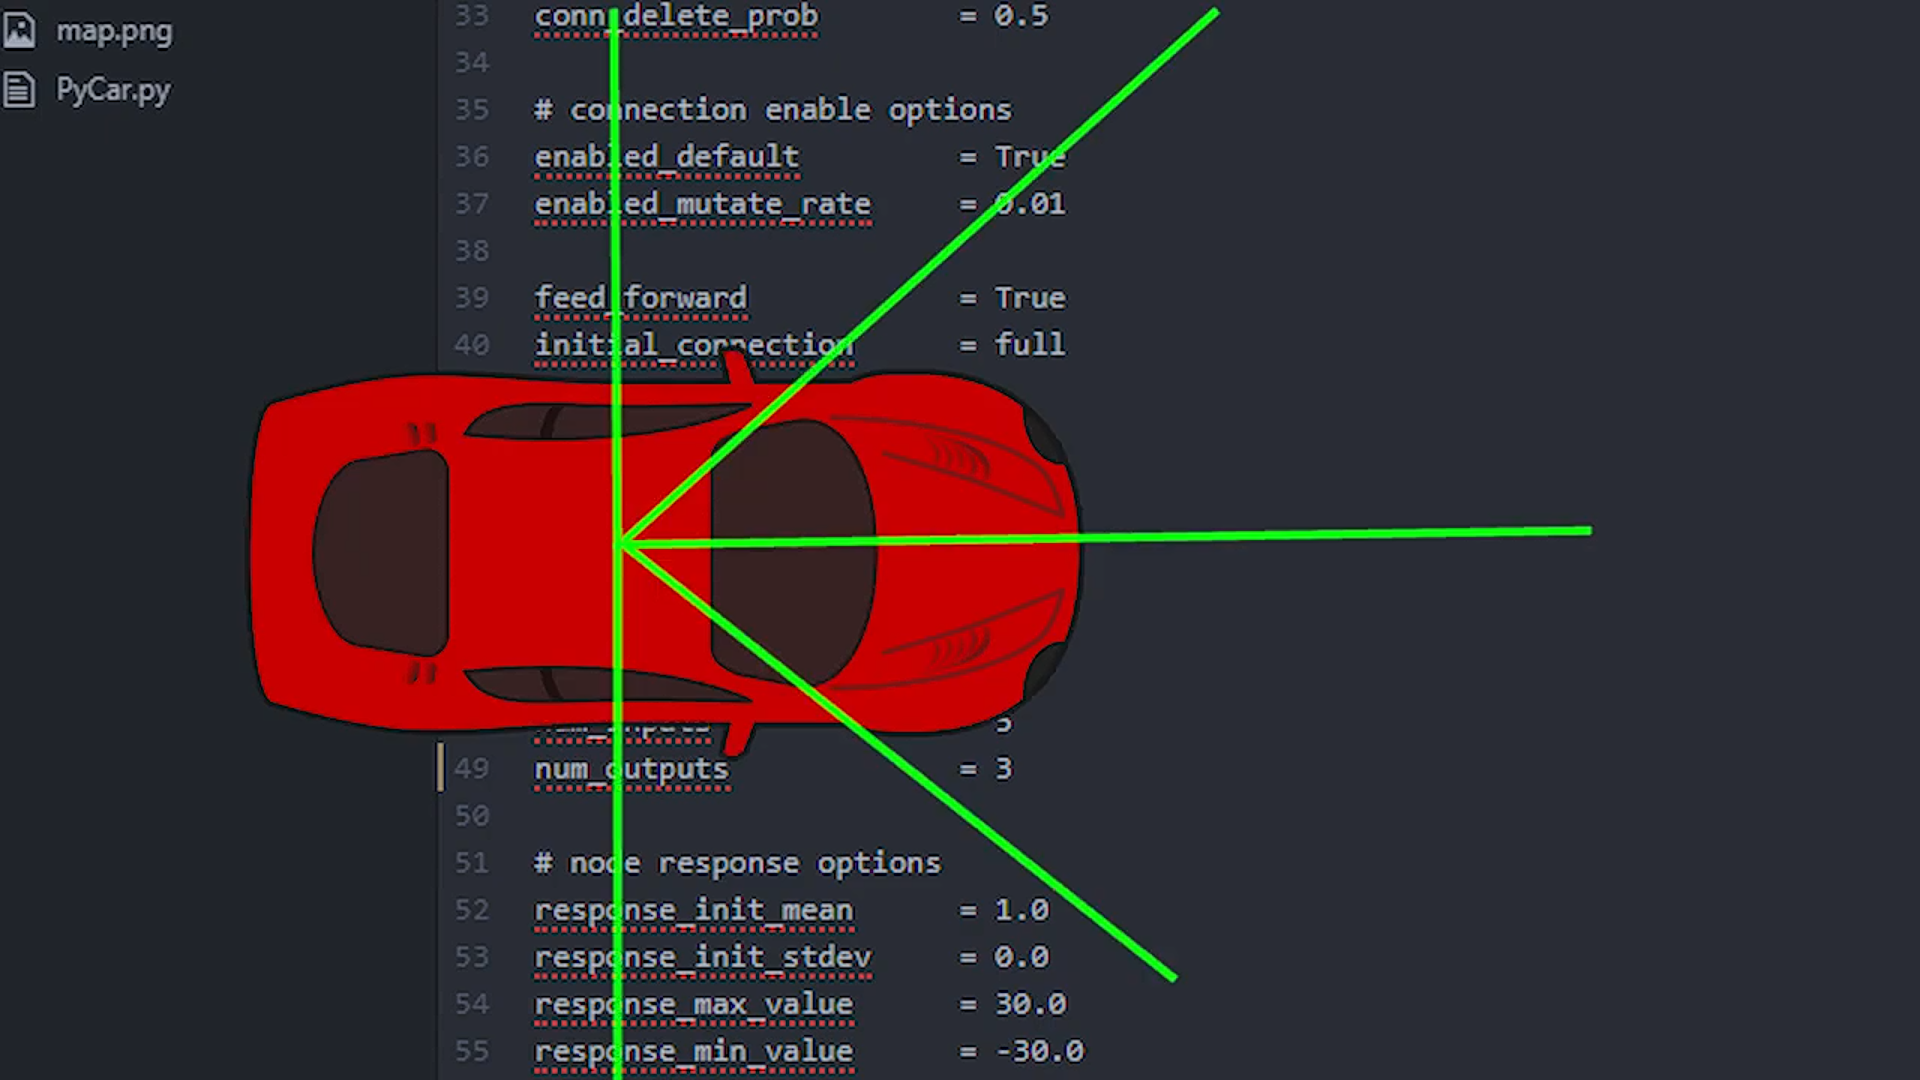
\includegraphics[width=0.7\linewidth]{images/car.png}
    \caption{project the reference channel Cheesy AI.}
    \label{fig:gym}
\end{figure}
\cite{Cheesy}

abaixo você pode encontra uma referência para mais informações. \textbf{config.txt}
\begin{lstlisting}[language=Python, caption=Detalhes de implementação do arquivo → \href{https://neat-python.readthedocs.io/en/latest/config_file.html}{config.txt} 
  \cite{neat-python}]
[NEAT]
fitness_criterion     = max
fitness_threshold     = 1000
pop_size              = 100
reset_on_extinction   = False

[DefaultGenome]
# node activation options
activation_default      = tanh
activation_mutate_rate  = 0.0
activation_options      = tanh

# node aggregation options
aggregation_default     = sum
aggregation_mutate_rate = 0.0
aggregation_options     = sum

# node bias options
bias_init_mean          = 0.0
bias_init_stdev         = 1.0
bias_max_value          = 30.0
bias_min_value          = -30.0
bias_mutate_power       = 0.5
bias_mutate_rate        = 0.7
bias_replace_rate       = 0.1

# genome compatibility options
compatibility_disjoint_coefficient = 1.0
compatibility_weight_coefficient   = 0.5

# connection add/remove rates
conn_add_prob           = 0.5
conn_delete_prob        = 0.5

# connection enable options
enabled_default         = True
enabled_mutate_rate     = 0.01

feed_forward            = True
initial_connection      = full

# node add/remove rates
node_add_prob           = 0.2
node_delete_prob        = 0.2

# network parameters
num_hidden              = 0
num_inputs              = 3
num_outputs             = 1

# node response options
response_init_mean      = 1.0
response_init_stdev     = 0.0
response_max_value      = 30.0
response_min_value      = -30.0
response_mutate_power   = 0.0
response_mutate_rate    = 0.0
response_replace_rate   = 0.0

# connection weight options
weight_init_mean        = 0.0
weight_init_stdev       = 1.0
weight_max_value        = 30
weight_min_value        = -30
weight_mutate_power     = 0.5
weight_mutate_rate      = 0.8
weight_replace_rate     = 0.1

[DefaultSpeciesSet]
compatibility_threshold = 3.0

[DefaultStagnation]
species_fitness_func = max
max_stagnation       = 20
species_elitism      = 2

[DefaultReproduction]
elitism            = 2
survival_thr
\end{lstlisting}
Abstração da implementação do projeto com Neat-Python
\begin{figure}[htpb!]
    \centering 
    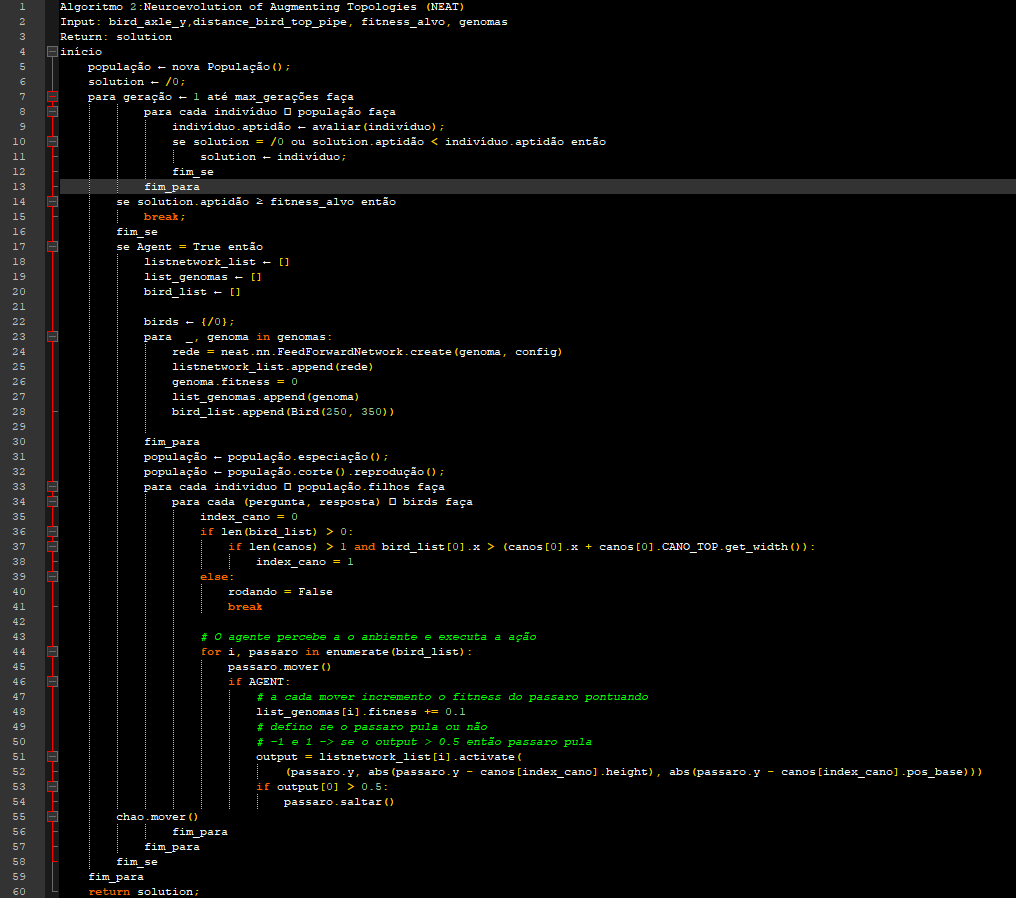
\includegraphics[width=0.7\linewidth]{images/abstract.png}
    \caption{abstração do projeto com Neat-Python}
    \label{fig:gym}
\end{figure}\\
Referência para detalhes do código 
\cite{mygit}
  

%



